\section{Punto de Vista de Contribución de Objetivos}
Contribución de objetivos es uno de los puntos de vista de la parte motivacional, este punto de vista permite profundizar y ahondar en los objetivos planteados en el proyecto, con el fin de precisar y aclarar las metas propuestas por medio de una especie de desglose de información. Esta contribución de objetivos como su nombre lo indica, no es única y exclusivamente de un solo objetivo, sino que por el contrario, dependiendo del caso y si hay objetivos relacionados entre si, se pueden agrupar en un solo paquete de objetivo para realizar esta contribución de una manera más personalizada y completa, procurando en todo momento la optimización de todos los recursos.

\subsection{Modelo de Contribución de Objetivos}
\begin{figure}[h!]
	\centering
	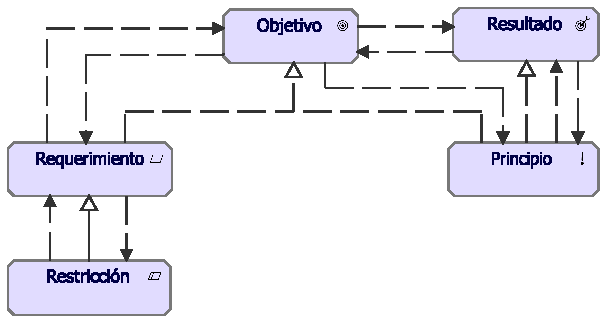
\includegraphics[width=1.0\linewidth]{imgs/modelo/ContObjetivos}
	\caption{Modelo Contribución de objetivos}
\end{figure}

El punto de vista de contribución de objetivos, presenta un modelo el cual como su nombre lo indica, se centra en un objetivo del proyecto planteado, del cual se desglosan ciertos requerimientos para este objetivo según sea el caso, sin dejar de mencionar que estos requerimientos pueden presentar en alguna ocasiones ciertas restricciones que son de vital importancia aclarar y mencionar para tener en cuenta en la estructuración del proyecto. Además de esto, siempre en cada modelo se busca un resultado o un fin específico, con este terminaría el punto de vista de contribución de objetivos.

%\newpage

\subsection{Caso  de Contribución de Objetivos}
\begin{figure}[h!]
	\centering
	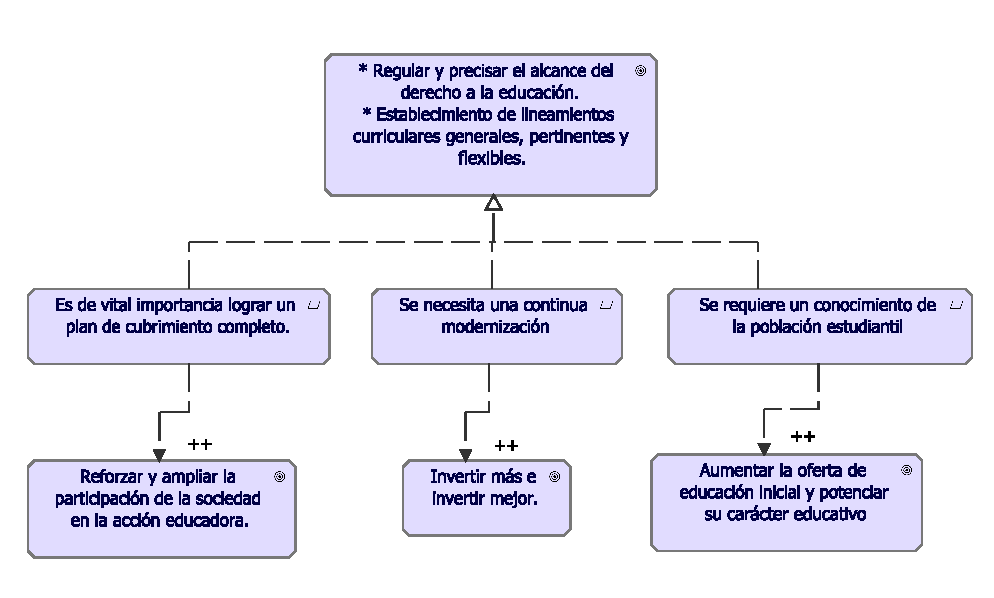
\includegraphics[width=1.0\linewidth]{imgs/motivacion/contriObjetivos/contriObjetivos.pdf}
	\caption{Caso Contribución de Objetivos}
\end{figure}

En el caso del proyecto planteado, en la sección de objetivos se postularon dos de estos, los cuales son transversales y están estrechamente relacionados, lo cual permite que se puedan trabajar al unisono, estos objetivos son: regular y precisar el alcance del derecho a la educación y establecimiento de lineamientos curriculares generales, pertinentes y flexibles. Ademas de esto, se plantearon tres requerimientos para estos objetivos, el primero de estos requerimientos se refiere a la importancia de lograr un plan de cubrimiento completo en educación para así cumplir con el objetivo de regular y precisar el alcance del derecho a la educación, el segundo requerimiento hace referencia a la modernización continua en la educación, para lo que se necesita más y mejor educación y finalmente, se encuentra el tercer requerimiento el cual indica la necesidad de un conocimiento de la población estudiantil con el fin de aumentar la oferta de educación inicial y potenciar su carácter educativo. De esta manera se realiza el punto de vista de contribución de objetivos, teniendo en cuenta los requerimientos a estos objetivos.
